\label{34-0430}
\section{Burnside and Polya}

\subsection{Burnside's Lemma}
\begin{lemma}1
    Given a set $S$ and a permutation group $G$ acting on $S$, the number of 
    equivalence classes of $S$ is given by $\frac 1{|G|}\sum_{\pi \in G}|\mathrm{fix}(\pi)|$. 
\end{lemma}
NOTE: in the above, $\pi$ is an operation on $S$, and $\mathrm{fix}(\pi)$ is the 
set of elements in $S$ \underline{fixed} by $\pi$. So, for a given $\pi$, count the 
elements in $S$ that do not change after that operation has been applied. 

\begin{example}1
    The square, $G = D_4$, $S$ = two-colorings of vertices of a square.
    Recall that $D_4$ is the \textit{dihedral group on four elements}. That is, 
    \[ G = e, r_1, r_2, r_3, V, H, L, R \]
    where $e$ is the identity, each lowercase $r$ represents a $90^\circ$-clockwise rotation
applied the number of times indicated by the subscript, $V$ is a vertical reflection,
 $H$ horizontal, $L$ across the left diagonal, and $R$ across the right. Let
us also say that the colors are red (R) and green (G).
\begin{center}
    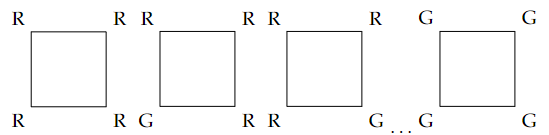
\includegraphics[scale=1]{figures/sqaure_colorings.png}
\end{center}
We can use Burnside's Lemma to find the number of equivalence groups. First,
let's make a table of all $\pi \in G$ and associated values for $|\mathrm{fix}(\pi)|$.
\begin{center}
    \begin{tabular}{c|c}
        $\pi$ & $|\mathrm{fix}(\pi)|$ \\ \hline
        $e$ & $2^4 = 16$ \\
        $r_1$ & 2 (all red, all green) \\
        $r_2$ & 4 (diagonals, all red, all green) \\
        $r_3$ & 2 (all red, all green) \\
        $V$ & 4 \\
        $H$ & 4 \\ 
        $L$ & 8 \\
        $R$ & 8 
    \end{tabular}
\end{center}
Now, we can use Burnside's: 
\[
    \frac 1{|G|}\sum_{\pi \in G}|\mathrm{fix}(\pi)| = 
    \frac 18 (16 + 2 + 4 + 2 + 4 + 4 + 8 + 8) = \boxed 6
\]
So, there are six (6) equivalence groups for $D_4$. 
\end{example}

\begin{example}2
    Bracelet with 5 beads and colored with red, blue, white, and
yellow. You can rotate but not flip the bracelet. How many distinct color-
ings are there?\\

Using Burnside's lemma:
\begin{center}
    \begin{tabular}{c|c}
        $\pi$ & $|\mathrm{fix}(\pi)|$ \\ \hline 
        $e$ & $4^5$ \\ 
        $r_1$ & 4 \\ 
        $r_2$ & 4 \\ 
        $r_3$ & 4 \\ 
        $r_4$ & 4 \\ 
    \end{tabular}
\end{center}
\[
    \frac 1{|G|}\sum_{\pi \in G}|\mathrm{fix}(\pi)| = 
    \frac 15 (4^5 + 4 \cdot 4) = 4^2 \times 13 = \boxed{208}
\]
\end{example}

\begin{example}3
    Same as Example 2, but you can reflect. 
    \begin{center}
        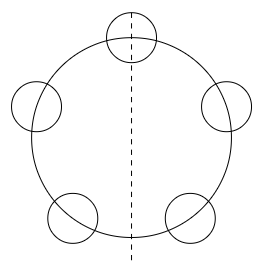
\includegraphics[scale=1]{figures/bracelet.png}
    \end{center}
    The above diagram shows an example of such a reflection. In total, there
    will be five (5) such reflections, bringing the total number of operations on
    the bracelet to ten (10).\\
      
    If we were to number the beads 1 through 5 clockwise from the top, the
    cycle notation for $R_1$, the illustrated reflection, would be $(1)(2 \ 5)(3 \ 4)$. 
    So, for all rotations $R_i$, $1 \leq i \leq 5$, $|\mathrm{fix}(R_i)| = 4^3$. 

    Apply Burnside's Lemma again, we get 
    \[
        \frac 1{|G|}\sum_{\pi \in G}|\mathrm{fix}(\pi)| = 
    \frac 1{10} (4^5 + 4 \cdot 4 + 5 \cdot 4^3) = 
    \frac 1{10} 4^2 \times 85 = \boxed{136}
    \]
 
\end{example}

\begin{example}4
    Let $G$ be the group of rotations of a cube. Write the elements
    of $G$ in cycle rotations.\\

    A cube has six faces, so there are three pairs of opposite faces. For a spindle
    going through the centres of two opposite faces there are two possible
    90 rotations, one going one way, one the other. This gives six 90 rotations.
    There is also a 180 rotation when the spindle goes through the centres of
    two opposite faces. This gives three further rotations.\\

    A cube also has twelve edges, so there are six pairs of opposite edges. For a
    spindle going through the centres of two opposite edges, the only possibility 
    is a rotation of 180. This gives six rotations, one for each pair of opposite
    edges. \\ 

    Finally a cube also has eight corners, so there are four pairs of opposite corners.
    For a spindle going through two opposite corners, there are two possible
     rotations, both of 120, one going one way, one the other. This means
    there are eight 120 rotations, two for each pair of opposite corners. \\

    We have counted 6+3+6+8 different rotations. Add the rotation by 0, which
        does nothing, and we have a group of \boxed{24} rotations.
\end{example}